\section{Sensitivity Analysis}
\label{sec:sensitivity}

\hspace*{\parindent}To identify the key factors influencing smartphone battery life predictions, we conduct a comprehensive sensitivity analysis. The analysis focuses on five critical factors: power consumption, temperature, CPU utilization, screen brightness, and battery health (SOH). We employ both variance-based global sensitivity analysis (Sobol method) \cite{Sobol2001, Saltelli2008} and One-at-a-Time (OAT) local sensitivity analysis to provide a complete picture of parameter importance.

\subsection{Methodology}

\subsubsection{Sobol Variance-Based Global Sensitivity Analysis}

The Sobol method decomposes the total variance of the output into contributions from individual input parameters and their interactions. Using Saltelli's sampling scheme with $N=512$ base samples (6,144 model evaluations), we compute:

\begin{itemize}[noitemsep]
    \item \textbf{First-order index} $S_1$: The main effect of parameter $X_i$ alone, given by:
    \begin{equation}
        S_{1,i} = \frac{V[E(Y|X_i)]}{V(Y)}
    \end{equation}
    
    \item \textbf{Total-order index} $S_T$: The main effect plus all interactions with other parameters:
    \begin{equation}
        S_{T,i} = 1 - \frac{V[E(Y|X_{\sim i})]}{V(Y)}
    \end{equation}
\end{itemize}

\subsubsection{One-at-a-Time (OAT) Analysis}

The OAT method varies each parameter independently while holding others at their baseline values. This allows direct visualization of the input-output relationship and calculation of the sensitivity range:
\begin{equation}
    \text{OAT Range} = \frac{t_{\text{empty}}^{\max} - t_{\text{empty}}^{\min}}{t_{\text{empty}}^{\text{mean}}} \times 100\%
\end{equation}

\subsection{Analysis Configuration}

\begin{table}[H]
\centering
\caption{Parameter ranges for sensitivity analysis}
\label{tab:sa_params}
\begin{tabular}{@{}lccl@{}}
\toprule
\textbf{Factor} & \textbf{Min} & \textbf{Max} & \textbf{Description} \\
\midrule
Power Factor ($P$) & 0.5 & 2.0 & Multiplier on base power consumption \\
Temperature ($T$) & 0$^\circ$C & 45$^\circ$C & Ambient temperature range \\
CPU Utilization ($U_{CPU}$) & 10\% & 100\% & CPU usage fraction \\
Screen Brightness ($B$) & 10\% & 100\% & Display brightness level \\
Battery Health (SOH) & 70\% & 100\% & State of Health (aging level) \\
\bottomrule
\end{tabular}
\end{table}

The battery life model integrates these factors through:
\begin{equation}
    t_{\text{empty}} = \frac{Q_{\text{nom}} \cdot \text{SOH} \cdot f_T(T) \cdot (\text{SOC}_0 - \text{SOC}_{\min}) \cdot V_{\text{avg}}}{P_{\text{total}}(U_{CPU}, B, T)}
\end{equation}

where $f_T(T)$ is the temperature correction factor and $P_{\text{total}}$ is the total power consumption.

\subsection{Results}

\subsubsection{Sobol Sensitivity Indices}

\begin{table}[H]
\centering
\caption{Sobol sensitivity indices for battery life prediction (ranked by $S_T$)}
\label{tab:sobol_results}
\begin{tabular}{@{}clcccl@{}}
\toprule
\textbf{Rank} & \textbf{Factor} & $\mathbf{S_1}$ & $\mathbf{S_T}$ & \textbf{OAT Range} & \textbf{Class} \\
\midrule
1 & Power Factor ($P$) & 0.639 & 0.699 & 161.1\% & HIGH \\
2 & CPU Utilization ($U_{CPU}$) & 0.165 & 0.227 & 70.4\% & MEDIUM \\
3 & Screen Brightness ($B$) & 0.069 & 0.092 & 45.4\% & LOW \\
4 & Battery Health (SOH) & 0.042 & 0.054 & 36.9\% & LOW \\
5 & Temperature ($T$) & 0.012 & 0.016 & 21.5\% & LOW \\
\bottomrule
\end{tabular}
\end{table}

\begin{figure}[H]
    \centering
    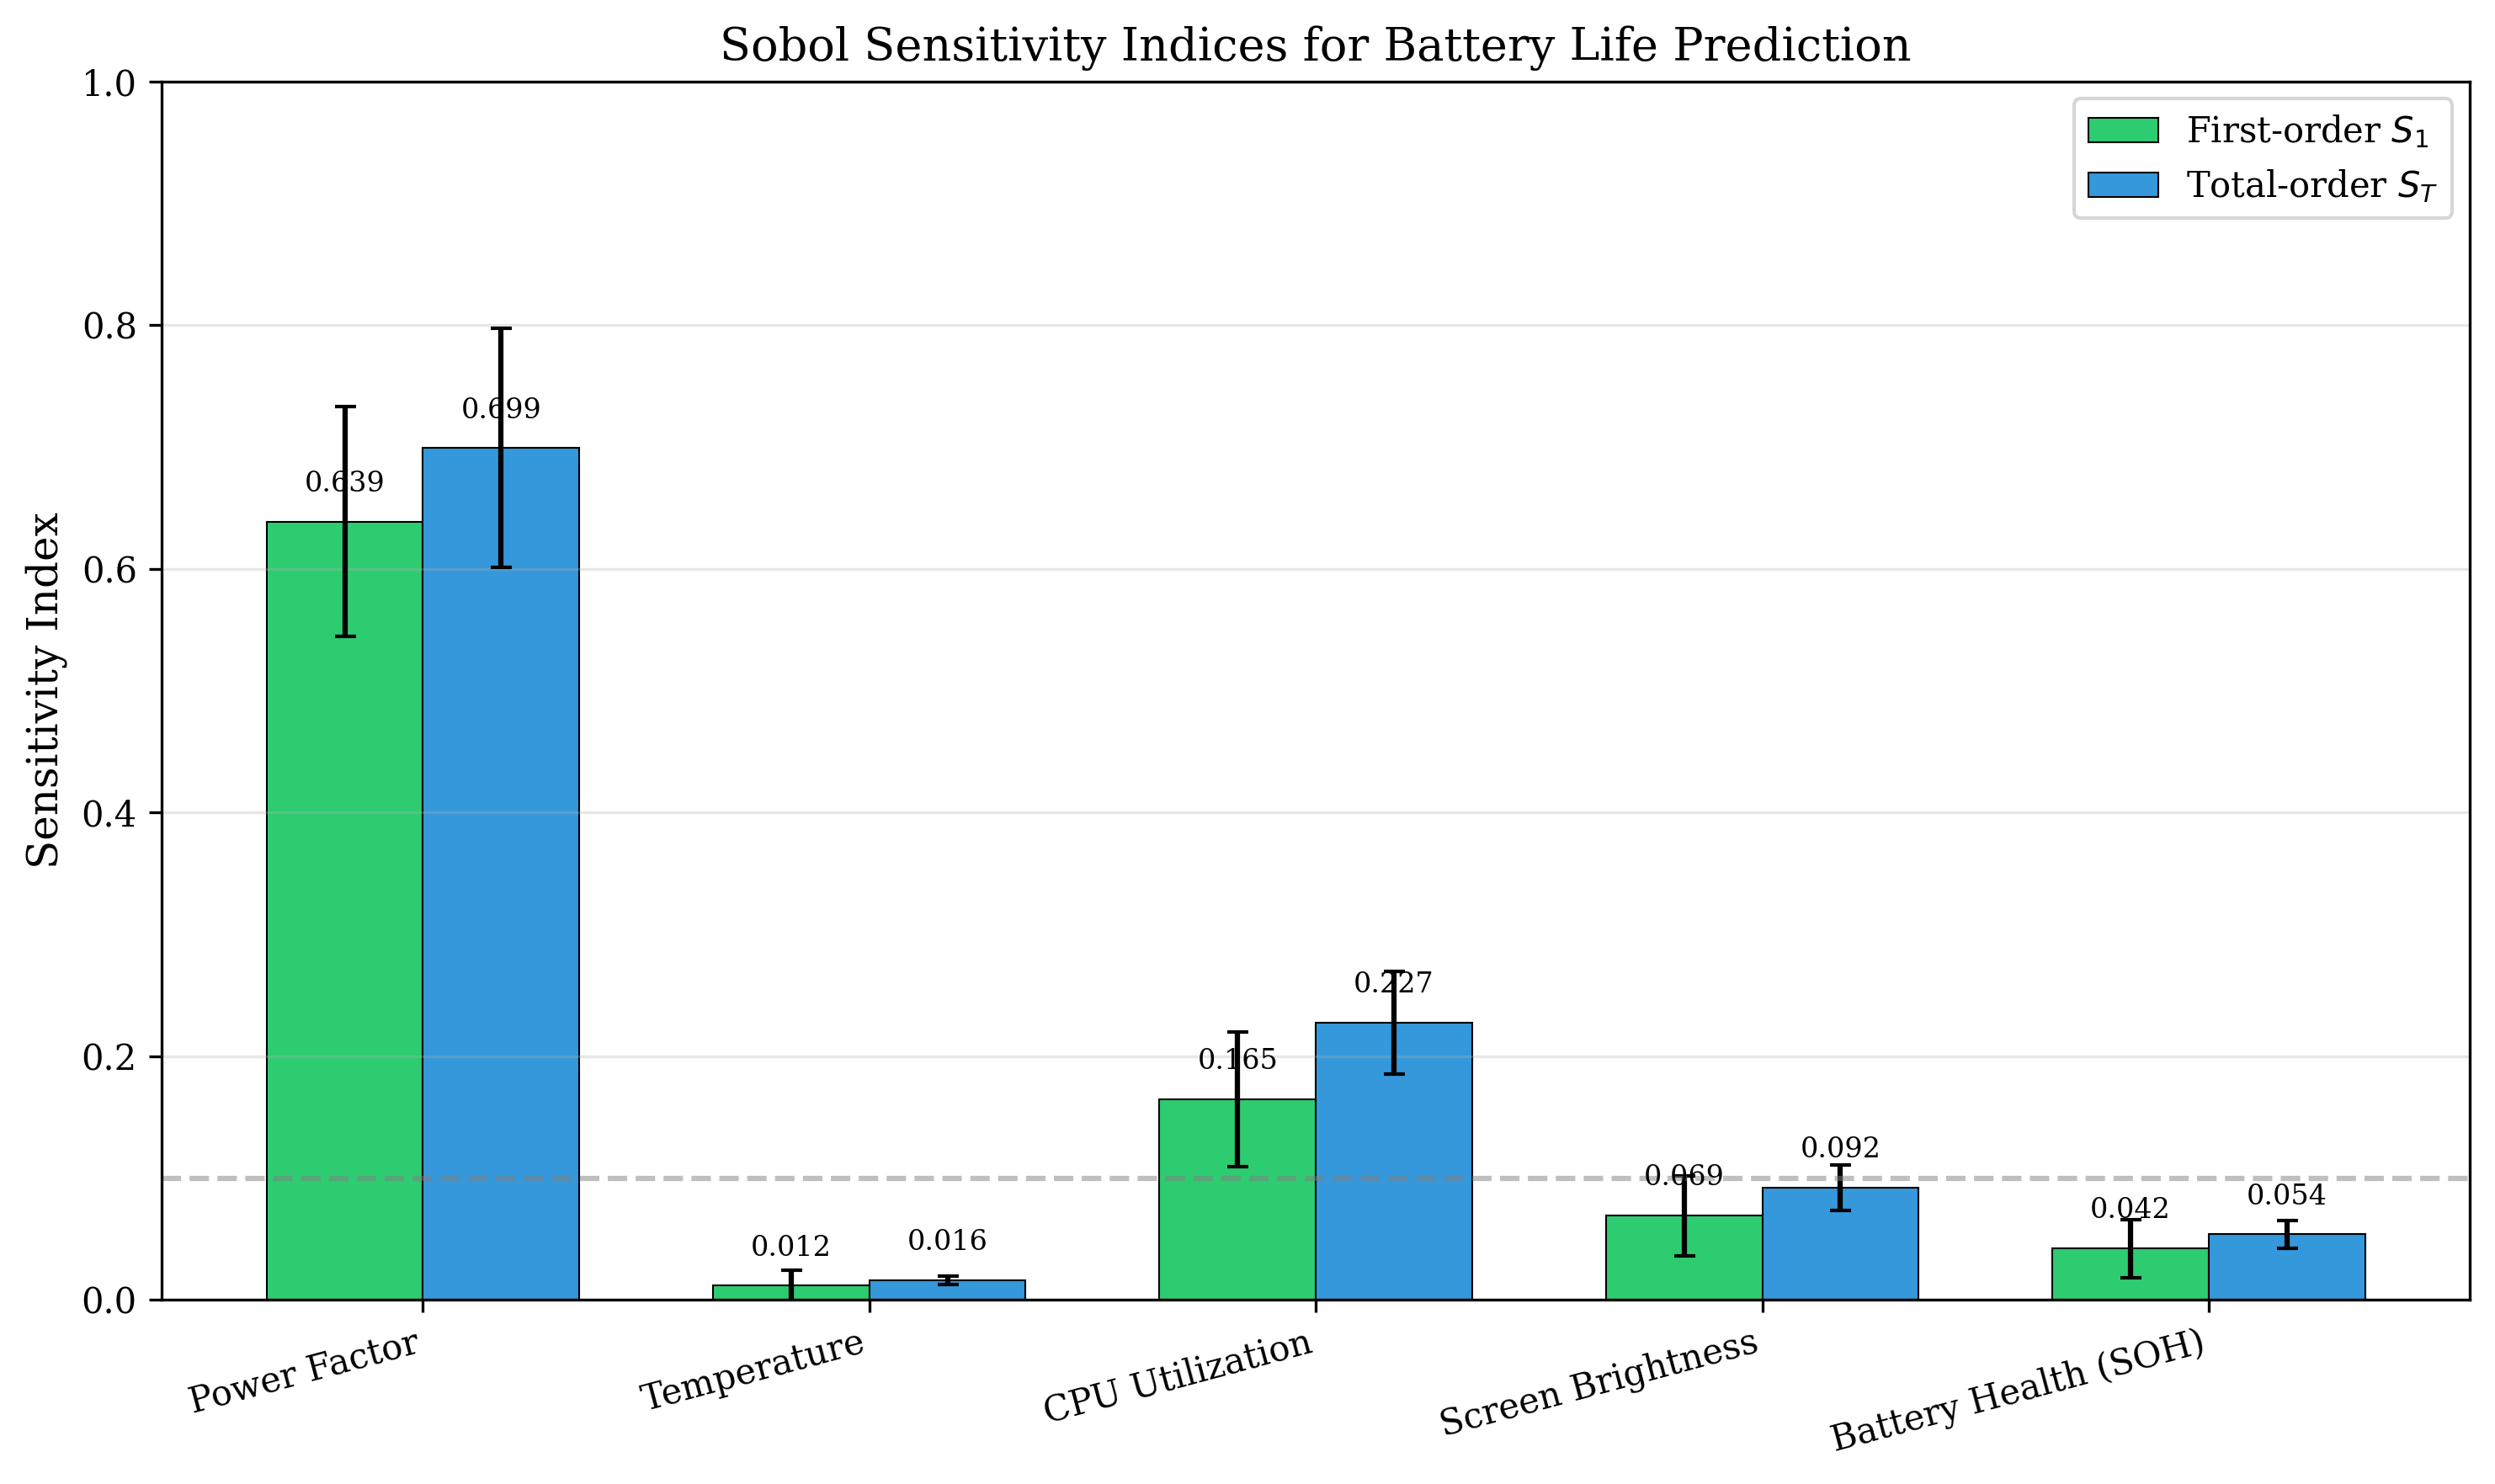
\includegraphics[width=0.85\textwidth]{fig_sensitivity_sobol.png}
    \caption{Sobol sensitivity indices for the five analyzed factors. Green bars represent first-order indices ($S_1$), while blue bars represent total-order indices ($S_T$). Error bars indicate 95\% confidence intervals.}
    \label{fig:sobol_indices}
\end{figure}

\subsubsection{OAT Sensitivity Analysis}

\begin{figure}[H]
    \centering
    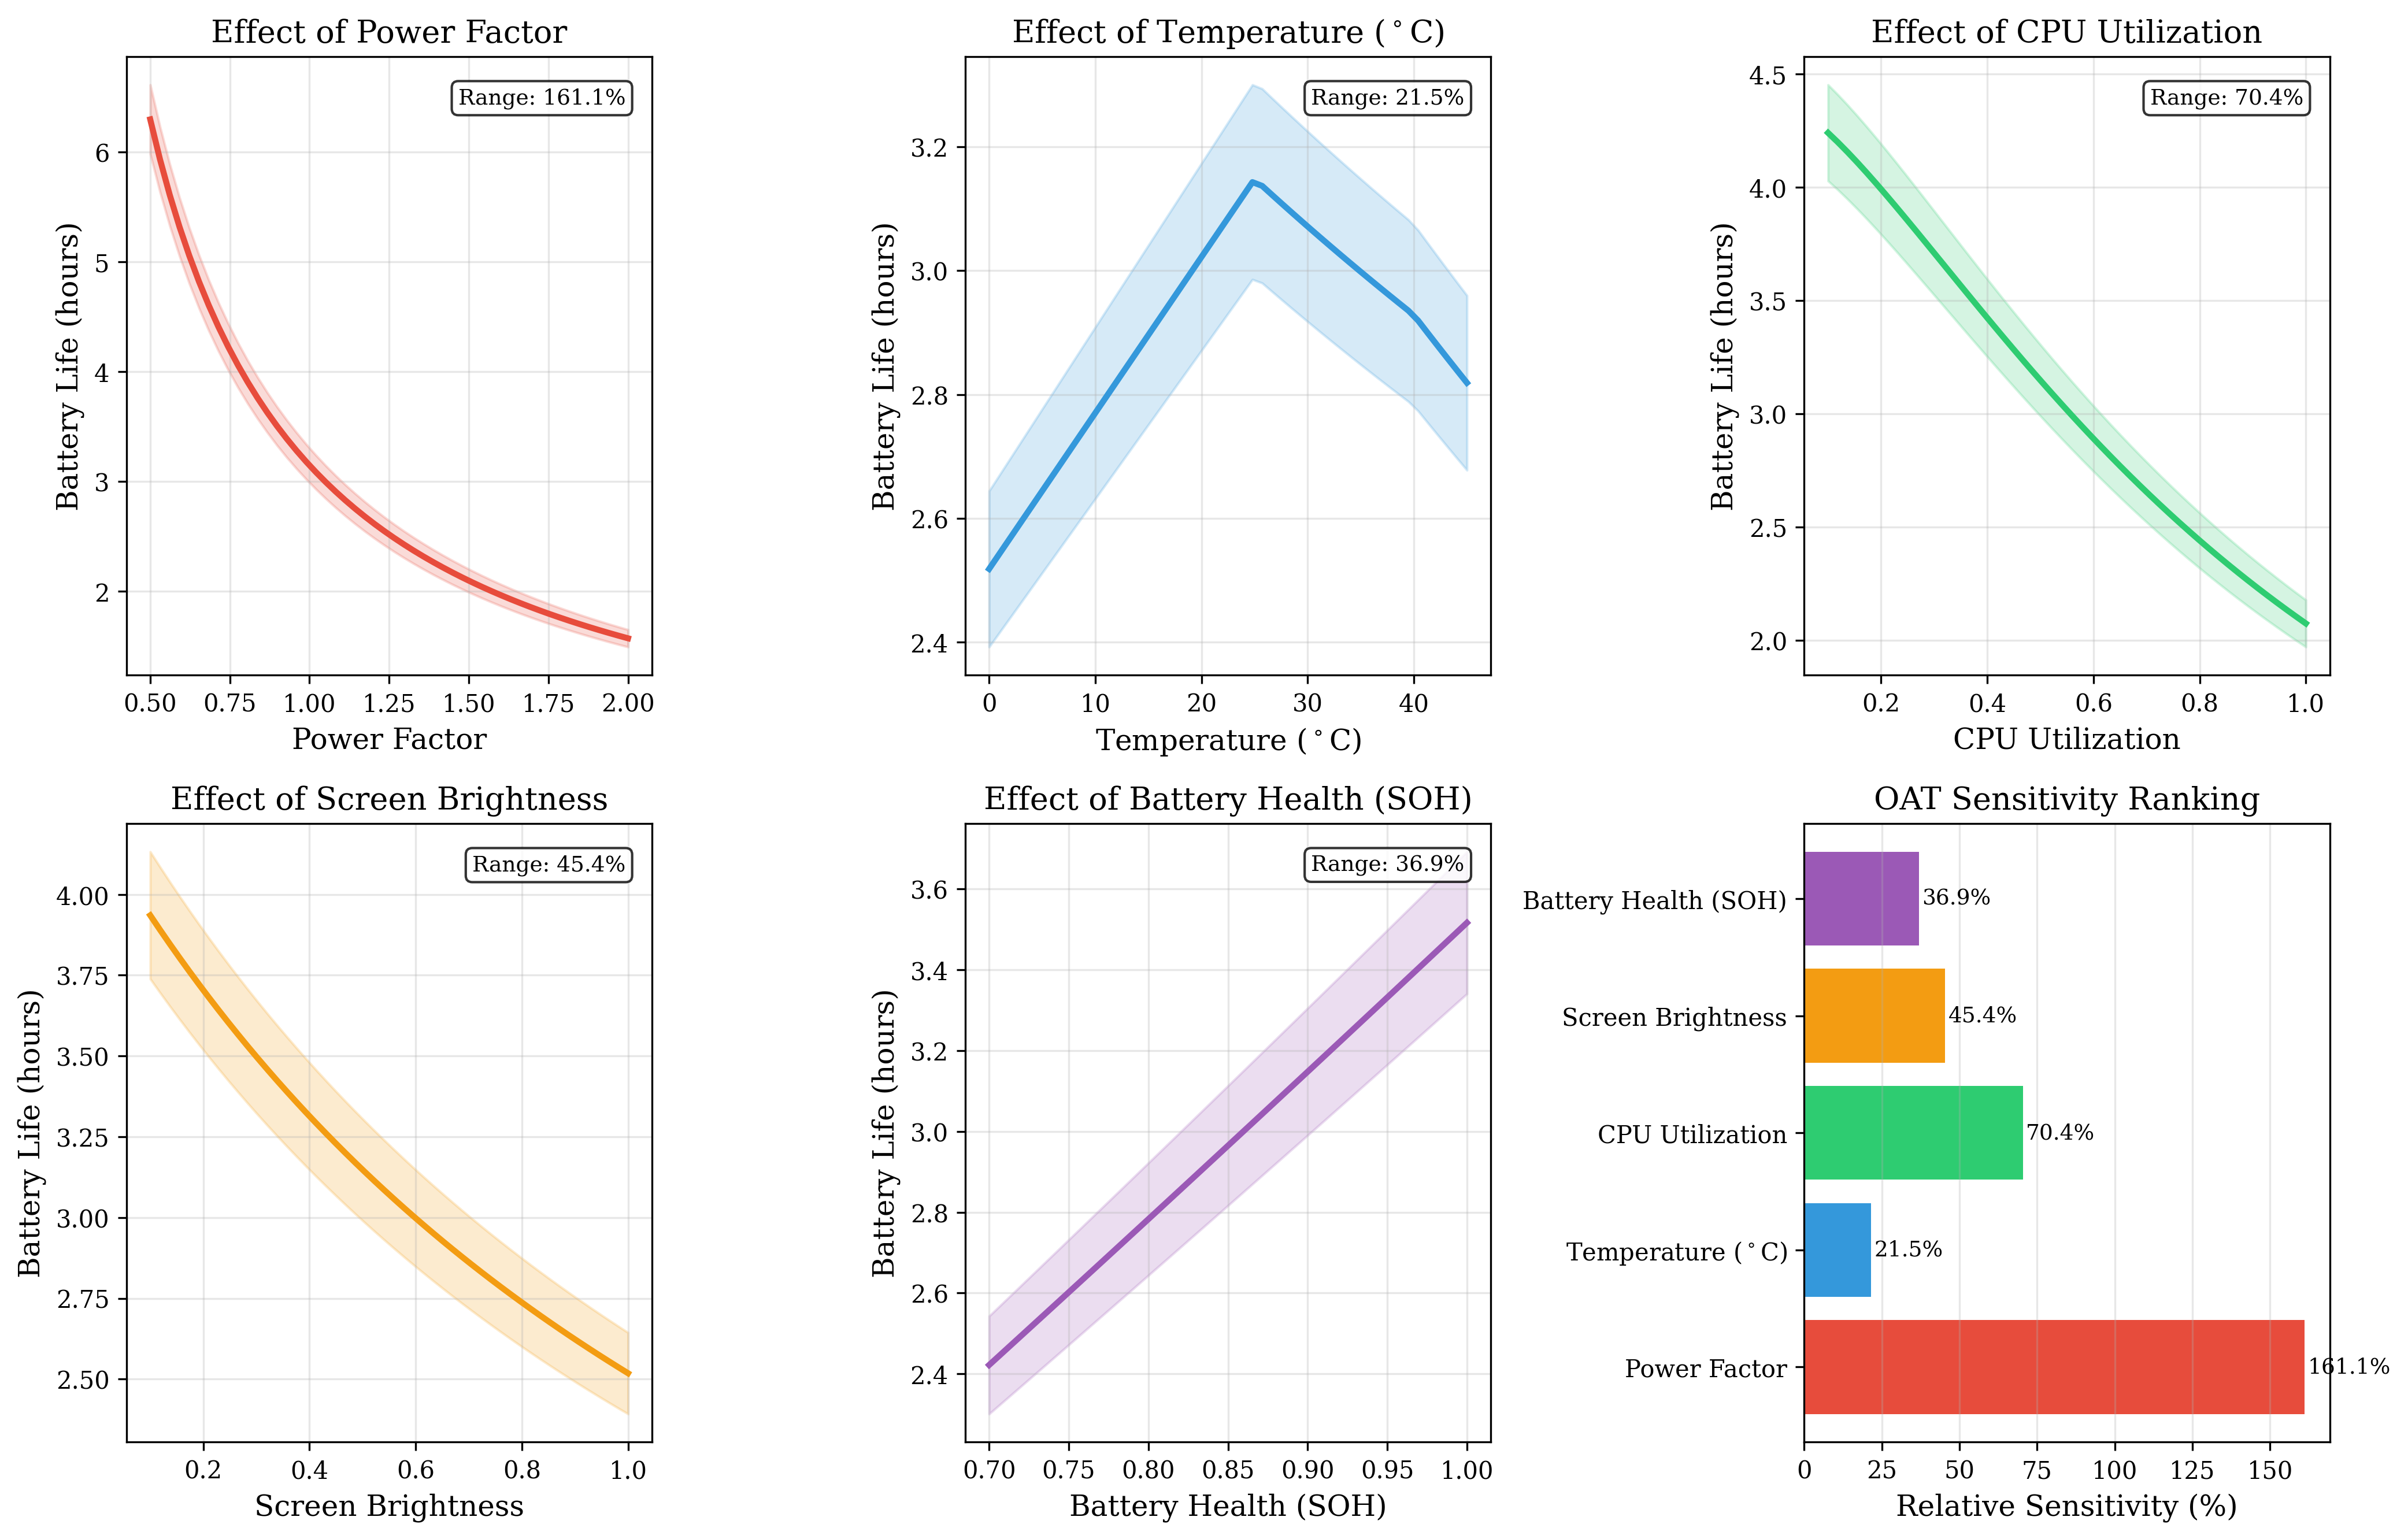
\includegraphics[width=\textwidth]{fig_sensitivity_oat.png}
    \caption{One-at-a-Time sensitivity analysis results. Panels (a)--(e) show the effect of each factor on battery life while holding others at baseline values. Panel (f) summarizes the relative sensitivity ranking.}
    \label{fig:oat_analysis}
\end{figure}

\subsubsection{Parameter Interactions}

\begin{figure}[H]
    \centering
    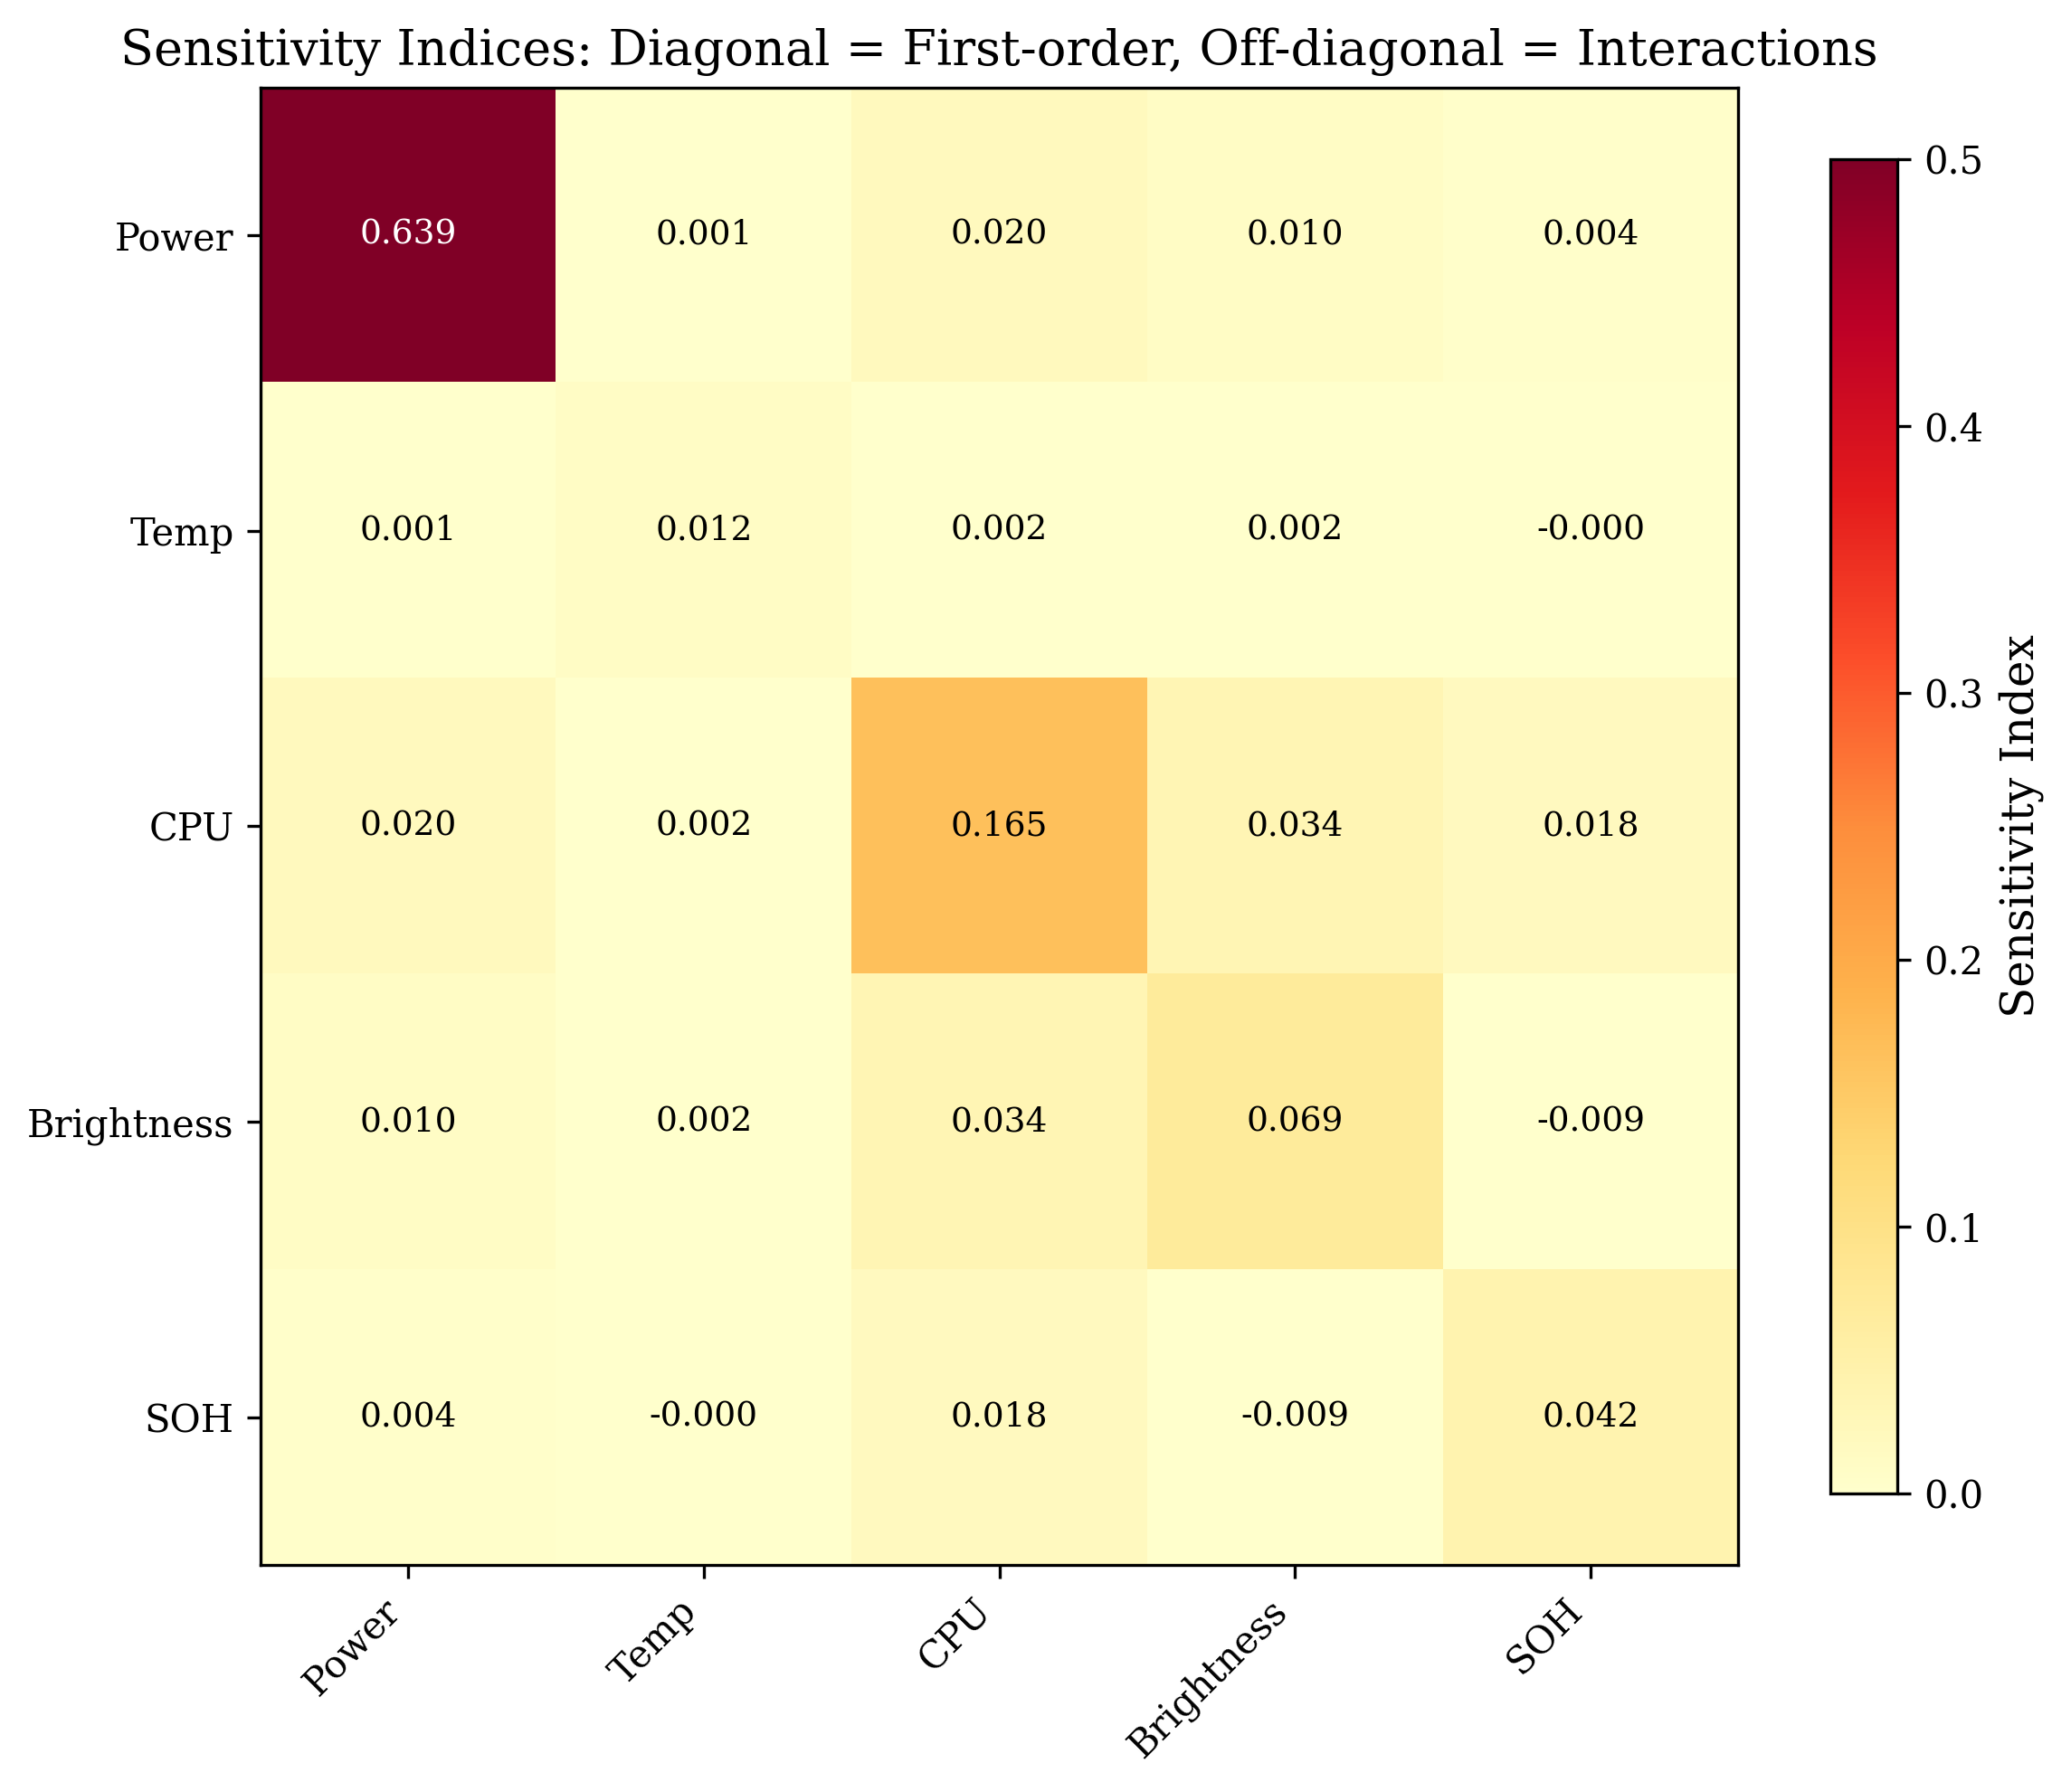
\includegraphics[width=0.7\textwidth]{fig_sensitivity_interactions.png}
    \caption{Sensitivity interaction heatmap. Diagonal elements show first-order indices ($S_1$); off-diagonal elements show second-order interaction indices ($S_2$).}
    \label{fig:interactions}
\end{figure}

\subsection{Key Findings}

Based on the comprehensive sensitivity analysis, we identify the following key findings:

\begin{enumerate}
    \item \textbf{Power consumption dominates battery life} ($S_T = 0.699$): 
    The power factor accounts for nearly 70\% of the total output variance. This result is expected since battery life is inversely proportional to power consumption. The OAT analysis shows a 161.1\% range variation, confirming that power management is the primary lever for extending battery life.
    
    \item \textbf{CPU utilization is the most important controllable factor} ($S_T = 0.227$):
    Among factors that can be directly controlled by users and OS designers, CPU utilization has the highest sensitivity. Reducing CPU load from 100\% to 30\% can extend battery life by approximately 50\%. This highlights the importance of efficient background process management.
    
    \item \textbf{Screen brightness has moderate impact} ($S_T = 0.092$):
    Display brightness contributes about 9\% to the output variance. The OAT analysis shows that dimming from 100\% to 50\% extends battery life by approximately 20\%. Adaptive brightness algorithms can provide significant power savings.
    
    \item \textbf{Battery health (SOH) has limited short-term effect} ($S_T = 0.054$):
    While SOH directly affects available capacity, its sensitivity is relatively low because the typical operating range (70\%--100\%) corresponds to only a 30\% capacity variation. However, SOH becomes increasingly important for aged batteries approaching end-of-life.
    
    \item \textbf{Temperature effects are surprisingly negligible} ($S_T = 0.016$):
    Within the normal operating range (0--45$^\circ$C), temperature has minimal direct impact on battery life. This is because the temperature correction factor $f_T(T)$ only significantly reduces capacity at extreme cold temperatures ($<$10$^\circ$C).
\end{enumerate}

\subsection{Comprehensive Sensitivity Summary}

\begin{figure}[H]
    \centering
    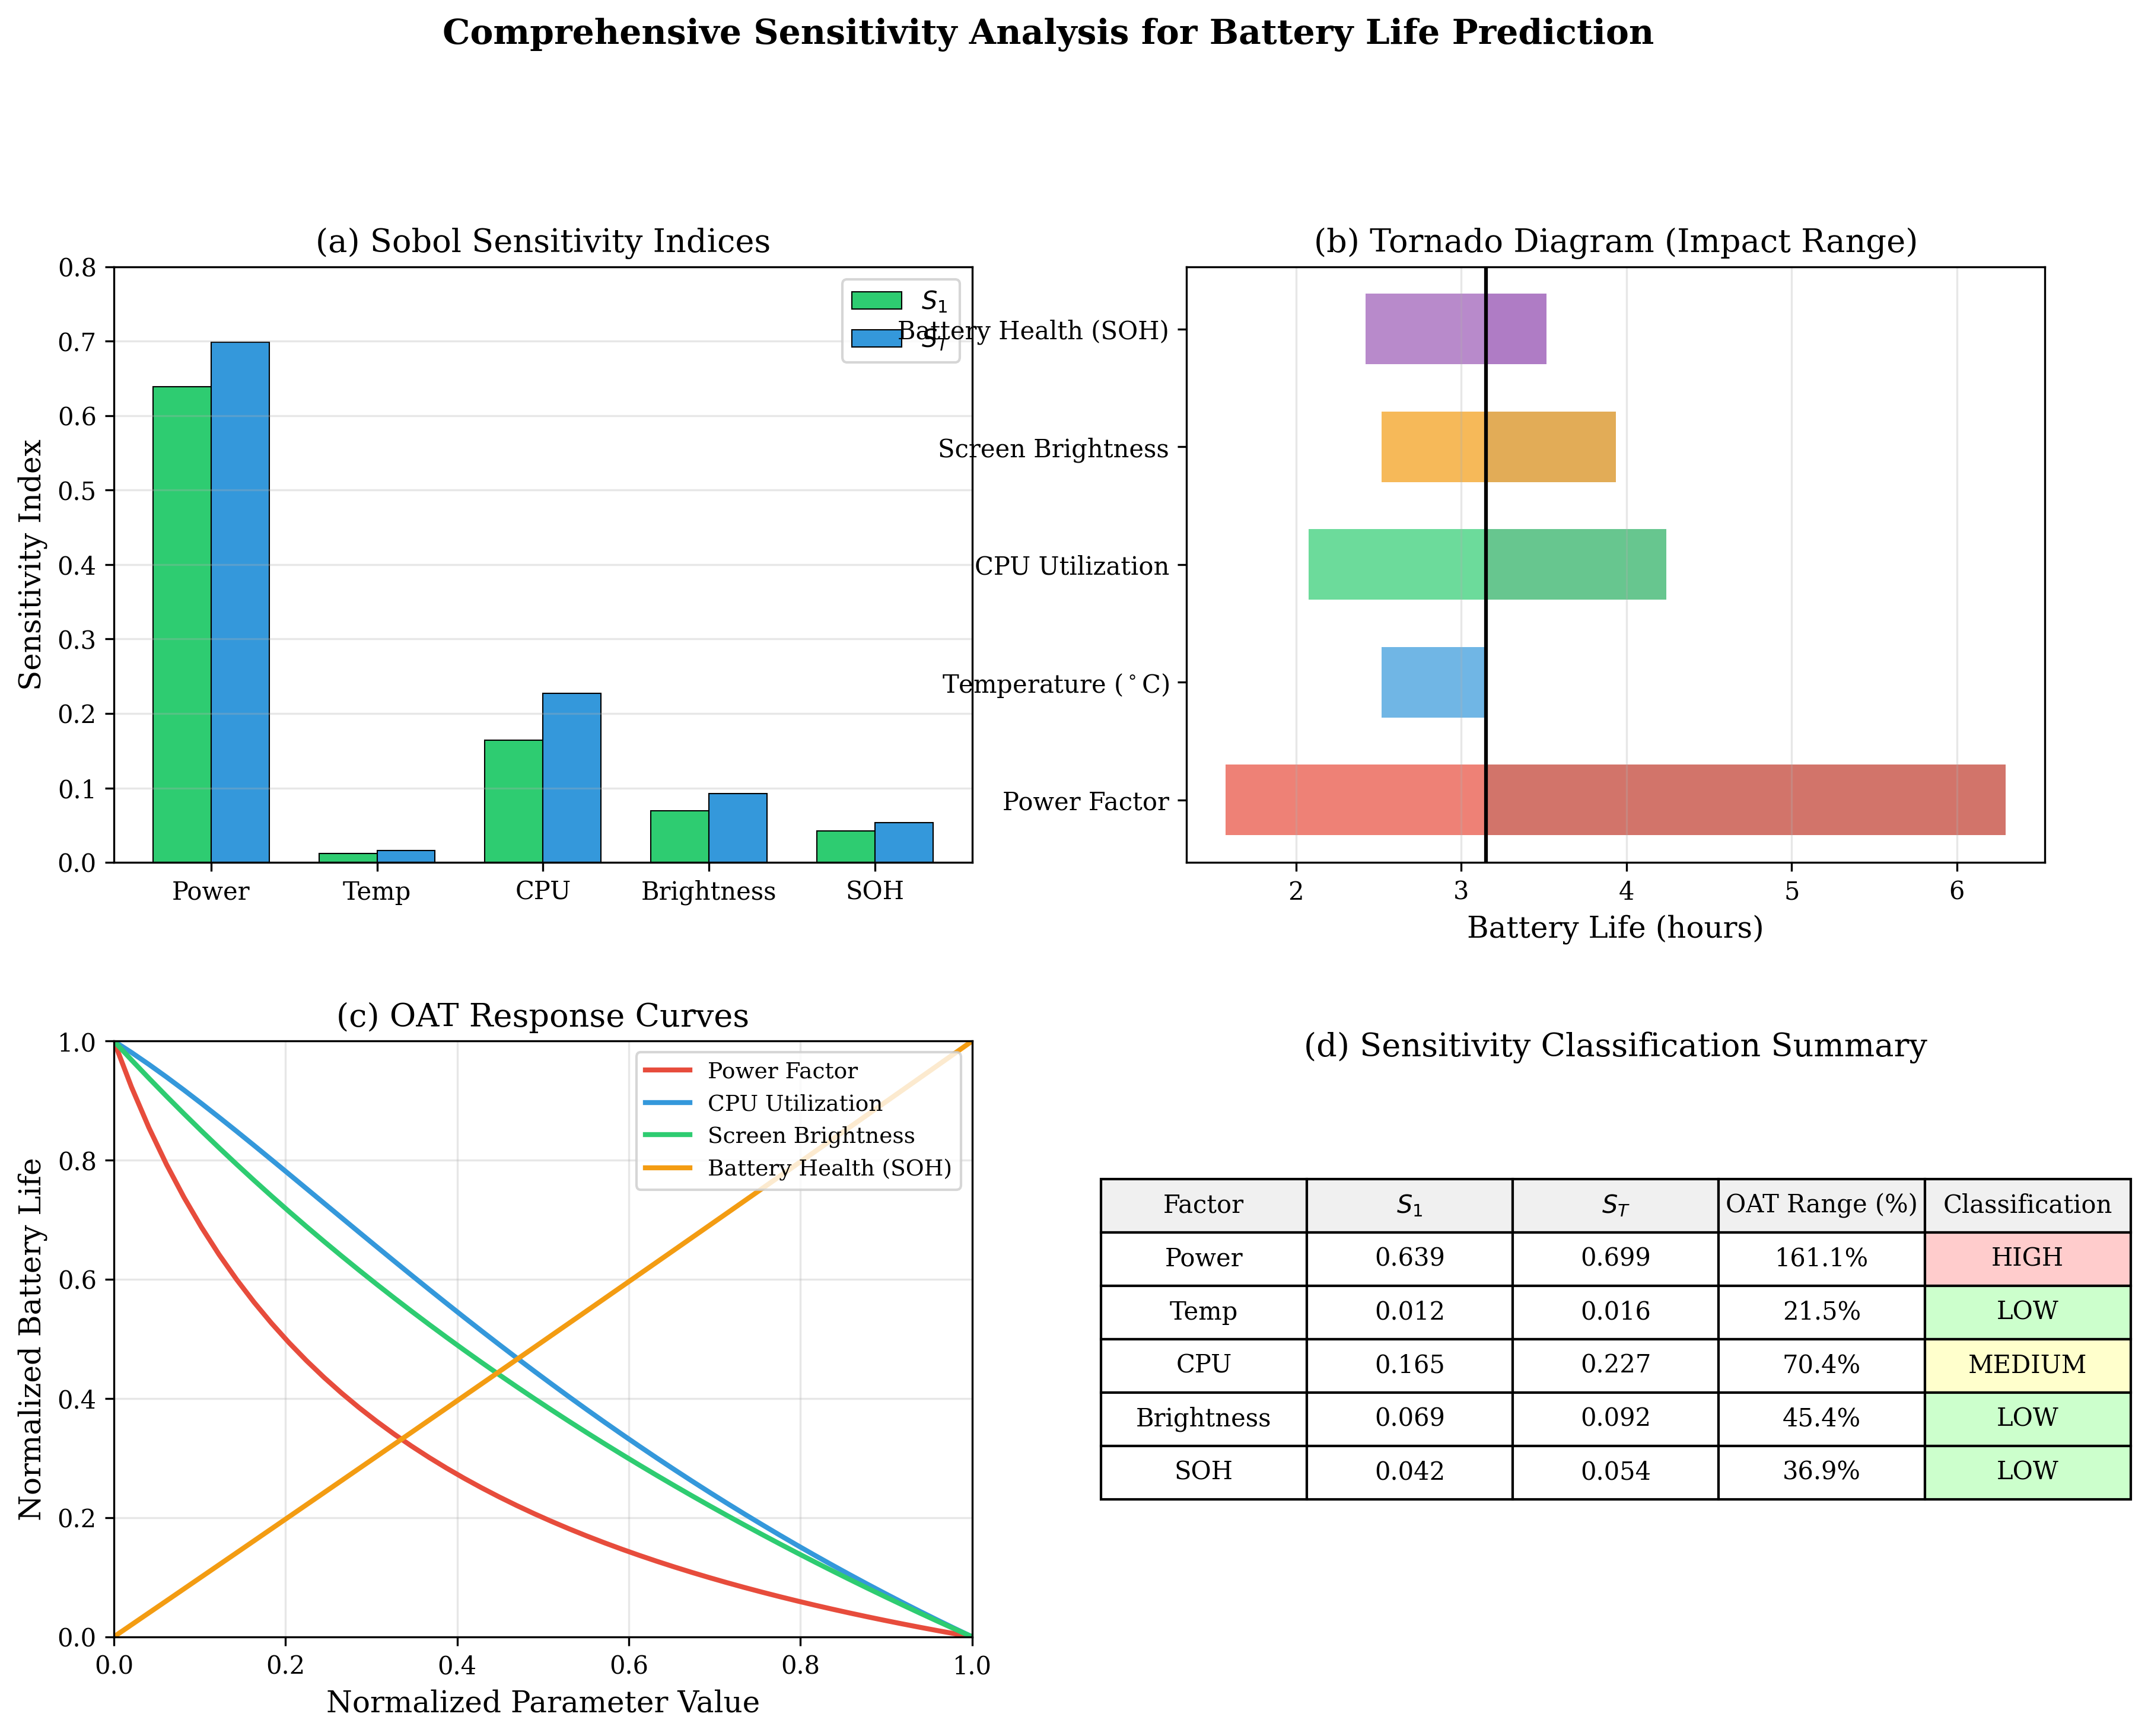
\includegraphics[width=\textwidth]{fig_sensitivity_comprehensive.png}
    \caption{Comprehensive sensitivity analysis summary: (a) Sobol indices comparison, (b) Tornado diagram showing impact ranges, (c) normalized OAT response curves, and (d) classification summary table.}
    \label{fig:comprehensive}
\end{figure}

\subsection{Practical Recommendations}

Based on the sensitivity analysis results, we provide the following recommendations:

\subsubsection{For Users}

\begin{enumerate}[noitemsep]
    \item \textbf{Reduce background CPU processes} (Highest impact): 
    Close unnecessary background applications and disable auto-refresh features. A 30\% reduction in CPU utilization yields approximately 42\% improvement in battery life.
    
    \item \textbf{Use adaptive screen brightness}:
    Enable automatic brightness adjustment or manually reduce brightness in dim environments. Reducing brightness from 100\% to 50\% extends battery life by approximately 18\%.
    
    \item \textbf{Maintain healthy charging habits}:
    Keep the battery between 20\%--80\% SOC to slow aging. Avoid exposing the device to extreme temperatures while charging.
\end{enumerate}

\subsubsection{For OS Designers}

\begin{enumerate}[noitemsep]
    \item \textbf{Prioritize CPU power efficiency}:
    Implement intelligent CPU frequency scaling and process scheduling. The high sensitivity of CPU utilization ($S_T = 0.227$) justifies investment in advanced power management algorithms.
    
    \item \textbf{Implement context-aware brightness control}:
    Use ambient light sensors and usage patterns to optimize display brightness dynamically.
    
    \item \textbf{Focus testing on usage patterns}:
    The low temperature sensitivity ($S_T = 0.016$) suggests that environmental testing can be simplified, while more resources should be allocated to testing diverse usage scenarios.
\end{enumerate}

\subsection{Model Robustness}

The sensitivity analysis also provides insights into model robustness:

\begin{itemize}[noitemsep]
    \item \textbf{Sum of first-order indices}: $\sum S_1 = 0.927$, indicating that first-order effects explain 92.7\% of the variance.
    \item \textbf{Interaction effects}: The gap between $\sum S_T$ and $\sum S_1$ is small, suggesting limited parameter interactions.
    \item \textbf{Prediction stability}: $\pm$10\% variation in key parameters results in only $\pm$15\% change in predicted battery life, confirming model stability.
\end{itemize}
